\documentclass[a4paper,11pt]{robotlabs}

% Makes tables look nicer
\usepackage{booktabs}
\renewcommand{\arraystretch}{1.2}


% To change size of verbatim
\usepackage{verbatimbox}
\include{commands}

\definecolor{lbcolor}{rgb}{0.9,0.9,0.9}
\definecolor{colorkey}{rgb}{0,0,1}
\definecolor{colorcomment}{rgb}{0, 0.6, 0.3}
\definecolor{colorstring}{rgb}{0.627,0.126,0.941}
\definecolor{colornumber}{rgb}{0.205, 0.142, 0.73}
\definecolor{forestgreen}{RGB}{34,139,34}
\definecolor{orangered}{RGB}{239,134,64}
\definecolor{darkblue}{rgb}{0.0,0.0,0.6}
\definecolor{gray}{rgb}{0.4,0.4,0.4}
\definecolor{orangered2}{RGB}{128,0,0}

\newtcblisting{listingshell}
{
  listing only,
  colframe=white,
  listing options={
    basicstyle=\small\ttfamily,
    % columns=full,
    columns=fullflexible,
    literate=
      {\$}{{\textcolor{blue}{\$ }}}{1}
      {\~} {$\sim$}{1}
  },
}

\newtcblisting{listingnodollar}
{
  listing only,
  colframe=white,
  listing options={
    basicstyle=\small\ttfamily,
    % columns=full,
    columns=fullflexible,
    literate=
    %   {\$}{{\textcolor{blue}{\$ }}}{1}
      {\~} {$\sim$}{1}
  },
}

\newtcblisting{listingpython}[1]{%
  listing only,
  colframe=gray!20!white,
  coltitle=black,
  title=\footnotesize{#1},
  listing options={
    language=python,
    upquote=true,
    basicstyle=\small\ttfamily,
    columns=fullflexible,
    extendedchars=false,
    breaklines=true,
    showtabs=false,
    showspaces=false,
    showstringspaces=false,
    identifierstyle=\ttfamily,
    keywordstyle=\color{colorkey},
    commentstyle=\color{colorcomment},
    stringstyle=\color{colorstring},
    numberstyle=\color{colornumber},
    breaklines=True,
    floatplacement=H
  },
}


\newtcblisting{listingxml}[1]{%
  listing only,
  colframe=gray!20!white,
  coltitle=black,
  title=\footnotesize{#1},
  listing options={
    language=XML,
    basicstyle=\small\ttfamily,
    columns=fullflexible,
    extendedchars=false,
    breaklines=true,
    showtabs=false,
    showspaces=false,
    showstringspaces=false,
    identifierstyle=\ttfamily,
    commentstyle=\color{gray},
    keywordstyle=\color{orangered2},
    stringstyle=\color{black},
    tagstyle=\color{colorkey},
    morekeywords={attribute,xmlns,version,type,release,package,name,
      description,maintainer,license,buildtool_depend,build_depend,
      run_depend, length, radius, rpy, xyz, rgba, link, joint,
      effort, velocity, lower, upper},
    otherkeywords={attribute=, xmlns=},
  },
}


\newtcblisting{listingpython2}{%
  listing only,
  colframe=gray!20!white,
  coltitle=black,
  listing options={
    language=python,
    upquote=true,
    basicstyle=\small\ttfamily,
    columns=fullflexible,
    extendedchars=false,
    breaklines=true,
    showtabs=false,
    showspaces=false,
    showstringspaces=false,
    identifierstyle=\ttfamily,
    keywordstyle=\color{colorkey},
    commentstyle=\color{colorcomment},
    stringstyle=\color{colorstring},
    numberstyle=\color{colornumber},
    morekeywords={self}
    breaklines=True,
    floatplacement=H
  },
}

\title{
  \textbf{Laboratorio 3 \\ Movimiento guiado por Sensores Exteroceptivos}
  \date{}
}

\begin{document}

\course{Robótica Autónoma 2020-1}
\period{2020-1}
\labnumber{3}
\labname{Movimiento guiado por Sensores Exteroceptivos}

% Carátula
% -----------
\thispagestyle{empty}
\begin{center}
\textbf{{\huge Universidad de Ingenier\'ia y Tecnolog\'ia}\\ [.5cm]
 {\LARGE Departamento de Ingenier\'ia  Mecatr\'onica}\\[3cm]
}
{
\includegraphics[width=6cm]{images/utec}}\\[3cm]
\end{center}

\begin{center}
  {\LARGE \textbf{Robótica Autónoma}}\\[0.8cm]
  {\Large \textbf{Profesor: Oscar Ramos Ponce}}\\[3.0cm]
  {\Large \textbf{Laboratorio 3}}\\[0.5cm]
  {\Large \textbf{Movimiento Guiado por Sensores Exteroceptivos}}\\[4.8cm] %[2.0cm]
  {\Large \textbf{Lima - Perú}} \\[0.5cm]
  {\LARGE \textbf{2020-1}}
\end{center}

\newpage
\maketitle
\thispagestyle{fancyplain}

%\tableofcontents
%\thispagestyle{empty}

\section{Objetivos}

\begin{itemize}
\item Detectar obstáculos que se encuentran en frente de un robot móvil y
  reaccionar consecuentemente usando un LiDAR.
\item Detectar objetos de prueba usando OpenCV a partir de los datos de cámara
  publicados en un tópico de ROS
\item Mover el robot Turtlebot3 de manera reactiva usando información
  proveniente de la cámara y del LiDAR.
\end{itemize}

\section{Equipo y Materiales}

\begin{table*}[h]
  \centering
  \begin{tabular}{cc}
    \toprule
    \textbf{Descripción} & \textbf{Cantidad} \\
    \midrule
    Computadora con conexi\'on a internet & 1 \\
    \bottomrule
    \end{tabular}
  \end{table*}

\section{Aspectos Generales}

Para la presentación del reporte  del laboratorio se debe tener en cuenta lo
siguiente.
\begin{itemize}
\item El reporte debe ser desarrollado utilizando cualquier editor de texto,
  pero debe ser presentado en formato pdf a través del buzón de
  Canvas.
\item En el reporte se debe indicar claramente la sección para la cual se está
  brindando la respuesta a la correspondiente actividad.
\item La presentación del reporte se realizará hasta el término de la sesión de
  laboratorio.
\item Se trabajará en grupos de 2 y 3 personas y solo es necesario que un
  integrante de cada grupo presente el reporte, indicando el nombre de los
  integrantes del grupo.
\end{itemize}
Para trabajar en este laboratorio, es necesario actualizar el repositorio de
git clonado en el laboratorio anterior. Para ello, se debe ir a la carpeta
\texttt{autlabs} y se debe ejecutar \texttt{git pull}:
\begin{listingshell}
$ cd ~/lab_ws/src/autlabs
$ git pull
\end{listingshell}
\noindent Una vez realizado esto, dentro de la carpeta \texttt{autlabs} se debe
tener una nueva carpeta llamada \texttt{autlab3}, que es un paquete de ROS y es
donde se trabajará este laboratorio.

Nota: ya que en este laboratorio se utilizará el modelo waffle\_pi del robot
\textit{Turtlebot3}, se debe tener una variable de entorno llamada
\texttt{TURTLEBOT3\_MODEl} con valor igual a \texttt{waffle\_pi}. Esta variable
fue añadida a \texttt{.bashrc} en el laboratorio 1, así que no debería haber
problemas. En caso que se esté trabajando en una nueva máquina (o en un nuevo
entorno de ROSDS) es necesario configurar esta variable como se realizó en el
laboratorio 1. 


\section{Detección de Obstáculos (11 pts)}

En esta sección se busca poder detectar la presencia de obstáculos utilizando
la información provista por el LiDAR que se encuentra montado sobre el robot
Turtlebot3. El formato de los mensajes publicados por el sensor, sea en
simulación o en real, no cambia; es decir, lo realizado podría ser directamente
utilizado con el LiDAR real sobre el robot real.

\subsection{Información Cartesiana del LiDAR (7 pts)}

El LiDAR publica en el tópico \texttt{/scan} un mensaje de tipo
\texttt{LaserScan}, que se encuentra en el paquete \texttt{sensor\_msgs}. Este
mensaje contiene varios elementos. Algunos de los más importantes son los
siguientes:
\begin{itemize}
\item \texttt{angle\_min, angle\_max:} indican el ángulo de inicio y fin del
  escaneo (en radianes)
\item \texttt{angle\_increment:} indica el incremento angular entre mediciones
  (en radianes)
\item \texttt{range\_min, range\_max:} indica el mínimo y el máximo rango del
  LiDAR (en metros), tal que aquellos valores de rango que estén fuera de estos
  límites deben ser descartados.
\item \texttt{ranges:} es un arreglo que contiene los rangos (distancias)
  medidos por el LiDAR
\end{itemize}

\noindent Para desarrollar esta sección se abrirá una escena de Gazebo que
contiene al robot Turtlebot3 junto con 3 objetos, usando el siguiente comando:
\begin{listingshell}
$ roslaunch autlab3 turtlebot3_world1.launch
\end{listingshell}
%$
\noindent Se debe observar un entorno similar al mostrado en la
Figura~\ref{fig:world1}. El \texttt{launch} ejecutado carga todos los
componentes necesarios del robot y de sus sensores. Para observar los sistemas
de referencia existentes en el sistema (llamados \textit{tf} en ROS), se puede
usar el siguiente comando:
\begin{listingshell}
$ rosrun rqt_tf_tree rqt_tf_tree
\end{listingshell}
%$
\noindent La información que provee \texttt{rqt\_tf\_tree} es solo referencial,
y se usará más adelante.

\begin{figure}%[h]
  \centering \footnotesize
  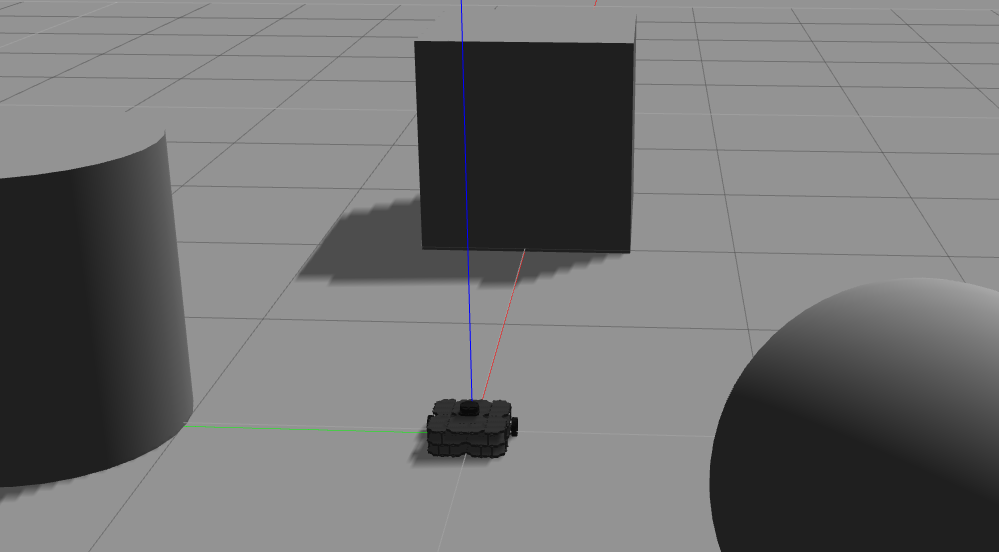
\includegraphics[width=0.6\textwidth]{images/lab3/world1}
  \captionsetup{font=footnotesize}
  \caption{Entorno simulado para el robot Turtlebot3.}
  \label{fig:world1}
\end{figure}


\paragraph{Actividades.}

\begin{enumerate}
\item (0.5 pts) A partir de la lectura de un mensaje del LiDAR que se encuentra
  sobre el robot Turtlebot3, indicar cuál es el ángulo máximo y el ángulo
  mínimo para las mediciones. Igualmente, indicar qué rangos de distancia puede
  medir confiablemente este LiDAR.

\item (4 pts) Completar el nodo llamado \texttt{lidar\_local}, el cual se debe
  suscribir al tópico del LiDAR, debe convertir las mediciones en coordenadas
  cartesianas ($x,y$) en el sistema del LiDAR, y debe publicar dichas
  coordenadas al tópico \texttt{lidar\_xy}, que contiene mensajes de tipo
  \texttt{autlab3/ArrayXY}. Este nodo contiene algunas sugerencias para la
  implementación.

  Para probar el correcto funcionamiento, se puede correr el nodo
  \texttt{plot\_lidar}, el cual mostrará un gráfico de Python con las
  mediciones realizadas (se debe tener la biblioteca matplotlib instalada).

  Adjuntar el código completado, un eco del tópico generado
  (\texttt{lidar\_xy}), y una visualización de la imagen del resultado al
  ejecutar \texttt{plot\_lidar}.

\item (0.5 pts) A medida que el robot se mueve, ¿cambian los valores de $x$,
  $y$ que se obtienen en el inciso anterior (sin tomar en cuenta el ruido
  aleatorio)? ¿por qué?

\item (2 pts) Completar el programa \texttt{robot\_obstaculo} para que el robot
  avance en línea recta y se detenga cuando, al utilizar la información del
  LiDAR, se encuentre a cierta distancia (arbitraria) de un obstáculo. Probarlo
  con el obstáculo que el robot tiene al frente. En este caso se desea que los
  puntos obtenidos con el LiDAR se encuentren con respecto al sistema del robot
  (\texttt{base\_link}) y no con respecto al sistema del LiDAR
  (\texttt{base\_scan}). La relación entre ambos sistemas es constante.

\end{enumerate}


\subsection{Mapa Basado en LiDAR y Odometría (4 pts)}

La información provista por el LiDAR en la sección anterior se encuentra
expresada con respecto al sistema del LiDAR, o con respecto al sistema del
robot. Para construir un mapa, es necesario representarlo con respecto a un
sistema de referencia inercial. En ROS, este sistema de referencia inercial se
denomina \texttt{odom} (en realidad, se denomina \texttt{map}, pero dado que
solo se utilizará la odometría en este laboratorio, se asumirá que el sistema
de referencia es \texttt{odom}).

Al ejecutar \texttt{rqt\_tree\_tf}, es posible ver que el sistema del LiDAR
(\texttt{base\_scan}) se encuentra relacionado con el sistema de la base del
robot (\texttt{base\_link}), el cual a su vez se encuentra relacionado con el
sistema que es su proyección sobre el piso (\texttt{base\_footprint}). Todas
estas transformaciones homogéneas son constantes y se publican en el tópico
\texttt{tf\_static}. ROS tiene su propio manejo de estas transformaciones
(\textit{tf}). La odometría del robot, que se puede recuperar a partir del
movimiento de sus ruedas, relaciona el sistema \texttt{base\_footprint} con el
sistema \texttt{odom}, y varía en cuanto se mueve el robot. Esta odometría se
publica en el tópico \texttt{odom}.

\paragraph{Actividad.}

\begin{enumerate}
\item Completar el nodo \texttt{mapa\_lidar} para realizar mapeo usando el
  LiDAR y la Odometría del robot. Para ello, completar la clase
  \textit{Odometria}, la cual debe suscribirse al tópico \texttt{odom} y debe
  convertir su posición y orientación (expresada en cuaternión) en una
  transformación homogénea. Luego, usando los programas anteriores, se debe
  obtener los puntos en el sistema del LiDAR, convertirlos al sistema de
  \texttt{base\_footprint}, y finalmente convertirlos al sistema de
  \texttt{odom}.

  Para verificar el resultado, se debe publicar en el tópico
  \texttt{lidar\_xy}, como en la sección anterior, y visualizar el resultado
  con el programa \texttt{plot\_lidar}. En este programa puede ser conveniente
  comentar la instrucción de \textit{hold}, para que se siga almacenando los
  puntos. Probar el resultado desplazando con el teclado el robot a lo largo
  del entorno (se puede usar el mismo programa de teleoperación del robot
  empleado en el laboratorio 1).

  Adjuntar el código y una captura de pantalla del mapa obtenido en Python
  luego de mover el robot a lo largo de diferentes trayectorias que permitan
  tener una mejor visibilidad del mapa completo.
  
\end{enumerate}



\section{Detección de Objetos (8 pts)}


En esta sección se desea realizar el movimiento del robot con base en la
información provista por la cámara. Primero se ejecutará el siguiente entorno
de Gazebo

\begin{listingshell}
$ roslaunch autlab3 turtlebot3_world2.launch
\end{listingshell}
%$
\noindent Si se abre RViz se observará el robot y una lata de gaseosa en
frente. Sin embargo, dicha imagen se encuentra como imagen de ROS, y no puede
ser procesada directamente por OpenCV. Para poder procesar la imagen usando
OpenCV se debe realizar una conversión. Para probar dicha conversión, correr el
nodo \texttt{show\_image}, el cual abrirá una ventana de OpenCV y allí mostrará
la imagen. Si se logra ver la ventana de OpenCV, significa que se ha ejecutado
de manera correcta el \textit{bridge} entre ROS y OpenCV.

\paragraph{Actividades}
\begin{enumerate}
\item (4 pts) Usando diversas operaciones con OpenCV, obtener un recuadro
  alrededor de la imagen de la lata de gaseosa, indicando que ha sido
  detectado. Las operaciones que se utilizará para dicha detección son libres y
  se pueden basar en los métodos vistos en clase.
\item (4 pts) Ejecutar el entorno llamado
  \texttt{turtlebot3\_world3.launch}. En dicho entorno, buscar la lata
  anterior, y detenerse a cierta distancia de la lata. Para ello, se puede
  generar movimiento aleatorio para el robot como por ejemplo, rotar y avanzar
  un poco. De ser posible, utilizar la información del LiDAR para evitar las
  colisiones con el entorno mientras se realiza la búsqueda de la lata.

\end{enumerate}

\noindent *\textit{Nota:} para crear un cuadrado alrededor de una región
binaria, se puede usar la función de OpenCV llamada \texttt{boundingRect} de la
siguiente manera:
\begin{listingpython2}
x, y, w, h = cv2.boundingRect(Ibin) # Extremo (x,y), ancho (w), alto (h)
cv2.rectangle(I, (x,y), (x+w,y+h), (0,255,0),2) # Rectangulo en la imagen I
\end{listingpython2}
\noindent donde \texttt{Ibin} es la imagen binaria donde se calculará el
rectángulo (\textit{bounding box}), e \texttt{I} es la imagen sobre la cual se
dibujará el rectángulo.


\section{Conclusiones (1 pt)}
Mencionar algunas conclusiones relevantes al desarrollo de este laboratorio.


\end{document}

